\chapter{Mengakses Basis Data NoSQL: mongoDB}

\section{Apa itu Basis Data NoSQL?}

\index{NOSQL}Pada awalnya, istilah NoSQL digunakan oleh Carlo Strozzi untuk menyebut nama software basis data yang dibuat olehnya. Software basis data tersebut tidak mengikuti standar SQL, sehingga dia menyebut software tersebut dengan "NoSQL"\footnote{\url{http://www.strozzi.it/cgi-bin/CSA/tw7/I/en_US/nosql/Home\%20Page}}. Setelah itu, istilah NoSQL dipopulerkan oleh Eric Evans untuk menyebut jenis software basis data yang tidak menggunakan standar SQL. Dalam perkembangan berikutnya, NoSQL ini lebih diarahkan pada "Not Only SQL" dan digunakan untuk kategorisasi basis data \textit{non-relational} (misalnya OODBMS, Graph Database, Document-oriented, dan lain-lain). Meski ada usaha untuk menstandarkan bahasa \textit{query} untuk NoSQL (UnQL - \textit{Unstructured Query Language}), sampai saat ini usaha tersebut tidak menghasilkan sesuatu hal yang disepakati bersama karena dunia NoSQL memang kompleks sekali. Untuk melihat daftar dari basis data NoSQL, anda bisa melihat ke \url{http://nosql-databases.org}.

\section{Mengenal mongoDB dan Fitur-fiturnya}

\index{mongoDB}mongoDB adalah salah satu software NoSQL yang termasuk dalam kategori \textit{Document Store} / \textit{Document-Oriented Database}, yaitu data disimpan dalam bentuk dokumen. Suatu dokumen bisa diibaratkan seperti suatu \textit{record} dalam basis data relasional dan isi dari masing-masing dokumen tersebut bisa berbeda-beda dan ada pula yang sama. Hal ini berbeda dengan basis data relasional yang menetapkan keseragaman kolom serta tipe data dengan data yang NULL jika tidak terdapat data. mongoDB menyimpan data dalam bentuk dokumen dengan menggunakan format JSON. Berikut adalah fitur dari mongoDB:
\begin{itemize}
	\item menggunakan format JSON dalam penyimpanan data
	\item mendukung indeks
	\item mendukung replikasi
	\item auto-sharding untuk skalabilitas horizontal
	\item query yang lengkap
	\item pembaruan data yang cepat
	\item mendukung Map/Reduce
	\item mendukung GridFS
\end{itemize}

\subsection{Memulai Server}
Seperti halnya basis data relasional seperti MySQL, PostgreSQL, dan lain-lain, mongoDB juga memulai dengan menjalankan server yang memungkinkan server tersebut melayani permintaan akses data dokumen melalui klien. Untuk memulai server, siapkan direktori yang akan menjadi tempat menyimpan data (defaultnya adalah /data/db). Jika menginginkan lokasi lain, gunakan argumen \textit{--dbpath} saat menjalankan server sebagai berikut (buat direktorinya jika belum ada):

\lstset{language=bash,caption=Menjalankan server MongoDB (mongod)}
\begin{lstlisting}
$ pwd
/home/bpdp/mongodb
$ mkdir data
$ mongod --rest --dbpath ./data
Tue Dec 11 14:40:20 
Tue Dec 11 14:40:20 warning: 32-bit servers don't have journaling 
enabled by default. Please use --journal if you want durability.
Tue Dec 11 14:40:20 
Tue Dec 11 14:40:20 [initandlisten] MongoDB starting : pid=24381 
port=27017 dbpath=./data 32-bit host=bpdp-arch
Tue Dec 11 14:40:20 [initandlisten] 
Tue Dec 11 14:40:20 [initandlisten] ** NOTE: when using MongoDB 
32 bit, you are limited to about 2 gigabytes of data
Tue Dec 11 14:40:20 [initandlisten] **       see 
http://blog.mongodb.org/post/137788967/32-bit-limitations
Tue Dec 11 14:40:20 [initandlisten] **       with --journal, the 
limit is lower
Tue Dec 11 14:40:20 [initandlisten] 
Tue Dec 11 14:40:20 [initandlisten] db version v2.2.2, pdfile 
version 4.5
Tue Dec 11 14:40:20 [initandlisten] git version: nogitversion
Tue Dec 11 14:40:20 [initandlisten] build info: Linux felix 
3.6.7-1-ARCH #1 SMP PREEMPT Sun Nov 18 10:11:22 CET 2012 i686 
BOOST_LIB_VERSION=1_50
Tue Dec 11 14:40:20 [initandlisten] options: { dbpath: "./data", rest: true}
Tue Dec 11 14:40:20 [initandlisten] Unable to check for journal 
files due to: boost::filesystem::directory_iterator::construct: 
No such file or directory: "./data/journal"
Tue Dec 11 14:40:21 [websvr] admin web console waiting for 
connections on port 28017
Tue Dec 11 14:40:21 [initandlisten] waiting for connections on 
port 27017
\end{lstlisting}

Untuk mengakhiri server, tekan \textit{Ctrl-C}, mongoDB akan mengakhiri server sebagai berikut:

\lstset{language=bash,caption=Mengakhiri server MongoDB (mongod)}
\begin{lstlisting}
^CTue Dec 11 15:16:38 got signal 2 (Interrupt), will terminate after current cmd ends
Tue Dec 11 15:16:38 [interruptThread] now exiting
Tue Dec 11 15:16:38 dbexit: 
Tue Dec 11 15:16:38 [interruptThread] shutdown: going to close listening sockets...
Tue Dec 11 15:16:38 [interruptThread] closing listening socket: 5
Tue Dec 11 15:16:38 [interruptThread] closing listening socket: 6
Tue Dec 11 15:16:38 [interruptThread] closing listening socket: 7
Tue Dec 11 15:16:38 [interruptThread] removing socket file: /tmp/mongodb-27017.sock
Tue Dec 11 15:16:38 [interruptThread] shutdown: going to flush diaglog...
Tue Dec 11 15:16:38 [interruptThread] shutdown: going to close sockets...
Tue Dec 11 15:16:38 [interruptThread] shutdown: waiting for fs preallocator...
Tue Dec 11 15:16:38 [interruptThread] shutdown: closing all files...
Tue Dec 11 15:16:38 [interruptThread] closeAllFiles() finished
Tue Dec 11 15:16:38 [interruptThread] shutdown: removing fs lock...
Tue Dec 11 15:16:38 dbexit: really exiting now
\end{lstlisting}

\subsection{Klien dan Shell mongoDB}

Setelah server hidup, pemrogram bisa menggunakan antarmuka administrasi web maupun menggunakan shell. \textit{Admin web console} bisa diakses menggunakan port 28017 seperti pada gambar~\ref{fig:mongowebadminconsole}. Sementara itu, untuk mengakses server menggunakan shell, bisa digunakan perintah \textit{mongo} sebagai berikut:

\lstset{language=bash,caption=Shell mongoDB (mongo)}
\begin{lstlisting}
$ mongo
MongoDB shell version: 2.2.2
connecting to: test
> 
\end{lstlisting}

  \begin{figure}
    \begin{center}
      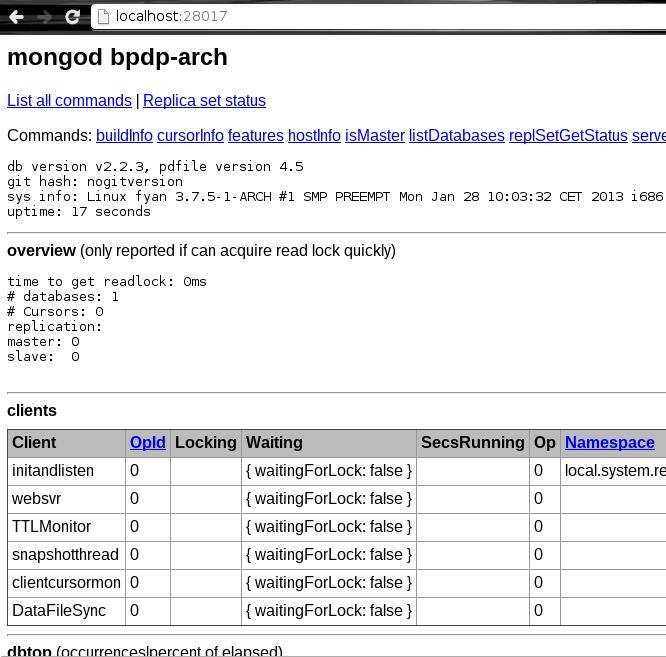
\includegraphics[scale=0.5]{images/mongodb-web-interface.jpg}
    \end{center}
    \caption{Admin web console untuk mongoDB}
    \label{fig:mongowebadminconsole}
  \end{figure}


\subsection{Documents dan Collections}

Konsep dasar yang harus dipahami dalam mongoDB sebagai \textit{document-oriented database} adalah \textit{documents} dan \textit{collections}. Sama halnya dengan basis data relasional, mongoDB menyimpan data dalam suatu basis data. Di dalam basis data tersebut terdapat \textit{collections} yang bisa diibaratkan seperti tabel dalam basis data relasional. \textit{Collections} digunakan untuk menyimpan dokumen (\textit{documents}). Dalam istilah basis data relasional, \textit{documents} adalah \textit{records}. Kerjakan latihan berikut untuk memahami pengertian dari \textit{documents} dan \textit{collections}.

\lstset{language=bash,caption=Sesi dalam shell mongoDB}
\begin{lstlisting}
$ mongo
MongoDB shell version: 2.2.2
connecting to: test
> db
test
> use mydb
switched to db mydb
> show dbs
local	(empty)
> emp1 = { name : "Zaky", address : "Griya Purwa Asri" }
{ "name" : "Zaky", "address" : "Griya Purwa Asri" }
> emp2 = { name : "Ahmad", address : "Purwomartani", email : "zakyahmadaditya@gmail.com" }
{
	"name" : "Ahmad",
	"address" : "Purwomartani",
	"email" : "zakyahmadaditya@gmail.com"
}
> emp3 = { name : "Aditya", address : "Kalasan", phone: "08787878787" }
{ "name" : "Aditya", "address" : "Kalasan", "phone" : "08787878787" }
> db.employees.insert( emp1 )
> db.employees.insert( emp2 )
> db.employees.insert( emp3 )
> show dbs
local	(empty)
mydb	0.0625GB
> db
mydb
> show collections
employees
system.indexes
> db.employees.find()
{ "_id" : ObjectId("50c74b63a7f83cba11e6b21e"), "name" : "Zaky", "address" : 
	"Griya Purwa Asri" }
{ "_id" : ObjectId("50c74b6da7f83cba11e6b21f"), "name" : "Ahmad", "address" : 
	"Purwomartani", "email" : "zakyahmadaditya@gmail.com" }
{ "_id" : ObjectId("50c74b79a7f83cba11e6b220"), "name" : "Aditya", "address" : 
	"Kalasan", "phone" : "08787878787" }
> db.employees.find( {name : "Ahmad"} )
{ "_id" : ObjectId("50c74b6da7f83cba11e6b21f"), "name" : "Ahmad", "address" : 
	"Purwomartani", "email" : "zakyahmadaditya@gmail.com" }
> db.employees.findOne()
{
	"_id" : ObjectId("50c74b63a7f83cba11e6b21e"),
	"name" : "Zaky",
	"address" : "Griya Purwa Asri"
}
> db.employees.find().limit(2)
{ "_id" : ObjectId("50c74b63a7f83cba11e6b21e"), "name" : "Zaky", "address" : 
	"Griya Purwa Asri" }
{ "_id" : ObjectId("50c74b6da7f83cba11e6b21f"), "name" : "Ahmad", "address" : 
	"Purwomartani", "email" : "zakyahmadaditya@gmail.com" }
> 
\end{lstlisting}

Basis data mongoDB hanya akan dibuat jika sudah dilakukan perintah untuk menyisipkan atau mengisikan data \textit{documents} ke dalam \textit{collections} seperti perintah di atas.

\section{Node.js dan MongoDB}

\subsection{Node-gyp}

\index{Node-gyp}Node-gyp merupakan \textit{native add-on build tool}, berfungsi untuk membantu proses kompilasi modul add-on native di Node.js. Node-gyp merupakan software bebas dan bisa diinstall menggunakan npm:

\lstset{language=bash,caption=Instalasi node-gyp}
\begin{lstlisting}
$ npm install -g node-gyp
npm http GET https://registry.npmjs.org/node-gyp
npm http 200 https://registry.npmjs.org/node-gyp
npm http GET https://registry.npmjs.org/glob
npm http GET https://registry.npmjs.org/mkdirp
npm http GET https://registry.npmjs.org/fstream
npm http GET https://registry.npmjs.org/minimatch
npm http GET https://registry.npmjs.org/graceful-fs
npm http GET https://registry.npmjs.org/request
npm http GET https://registry.npmjs.org/tar
npm http GET https://registry.npmjs.org/semver
npm http GET https://registry.npmjs.org/rimraf
npm http GET https://registry.npmjs.org/which
npm http GET https://registry.npmjs.org/osenv
npm http GET https://registry.npmjs.org/npmlog
npm http GET https://registry.npmjs.org/nopt
npm http 304 https://registry.npmjs.org/glob
npm http 304 https://registry.npmjs.org/minimatch
npm http 304 https://registry.npmjs.org/mkdirp
npm http 304 https://registry.npmjs.org/request
npm http 304 https://registry.npmjs.org/graceful-fs
npm http 304 https://registry.npmjs.org/semver
npm http GET https://registry.npmjs.org/semver/-/semver-1.1.1.tgz
npm http 200 https://registry.npmjs.org/fstream
npm http 200 https://registry.npmjs.org/tar
npm http GET https://registry.npmjs.org/tar/-/tar-0.1.14.tgz
npm http 200 https://registry.npmjs.org/rimraf
npm http 200 https://registry.npmjs.org/which
npm http 304 https://registry.npmjs.org/nopt
npm http 200 https://registry.npmjs.org/osenv
npm http 200 https://registry.npmjs.org/npmlog
npm http 200 https://registry.npmjs.org/semver/-/semver-1.1.1.tgz
npm http 200 https://registry.npmjs.org/tar/-/tar-0.1.14.tgz
npm http GET https://registry.npmjs.org/abbrev
npm http GET https://registry.npmjs.org/sigmund
npm http GET https://registry.npmjs.org/lru-cache
npm http GET https://registry.npmjs.org/ansi
npm http GET https://registry.npmjs.org/inherits
npm http GET https://registry.npmjs.org/inherits
npm http GET https://registry.npmjs.org/inherits
npm http GET https://registry.npmjs.org/block-stream
npm http 304 https://registry.npmjs.org/sigmund
npm http 304 https://registry.npmjs.org/abbrev
npm http 304 https://registry.npmjs.org/lru-cache
npm http 304 https://registry.npmjs.org/inherits
npm http 304 https://registry.npmjs.org/inherits
npm http 304 https://registry.npmjs.org/inherits
npm http 200 https://registry.npmjs.org/ansi
npm http 200 https://registry.npmjs.org/block-stream
/home/bpdp/software/nodejs/bin/node-gyp -> /home/bpdp/software/nodejs/lib/node_modules/
	node-gyp/bin/node-gyp.js
node-gyp@0.8.1 /home/bpdp/software/nodejs/lib/node_modules/node-gyp
+-- graceful-fs@1.1.14
|-- osenv@0.0.3
|-- rimraf@2.0.2
|-- mkdirp@0.3.4
|-- which@1.0.5
|-- semver@1.1.1
|-- request@2.9.203
|-- nopt@2.0.0 (abbrev@1.0.3)
|-- minimatch@0.2.9 (sigmund@1.0.0, lru-cache@2.0.4)
|-- glob@3.1.14 (inherits@1.0.0)
|-- fstream@0.1.19 (inherits@1.0.0)
|-- npmlog@0.0.2 (ansi@0.1.2)
+-- tar@0.1.14 (inherits@1.0.0, block-stream@0.0.6)
\end{lstlisting}

Node-gyp ini diinstall pada lokasi global. Pada materi ini, Node-gyp diperlukan untuk membangun \textit{driver} dari mongoDB sehingga mongoDB bisa diakses oleh Node.js. 

\subsection{Driver Node.js untuk mongoDB}

\index{mongoDB!Driver}Mengakses mongoDB dari Node.js bisa dilakukan dengan menggunakan driver atau berbagai \textit{wrapper} serta solusi sejenis ORM \textit{Object-Relational Mapping}. Beberapa solusi yang tersedia adalah:
\lstset{language=bash,caption=Instalasi driver mongoDB}
\begin{lstlisting}
$ npm install mongodb
npm WARN package.json kintamani@0.1.0 No README.md file found!
npm http GET https://registry.npmjs.org/mongodb
npm http 304 https://registry.npmjs.org/mongodb
npm http GET https://registry.npmjs.org/bson/0.1.5
npm http 304 https://registry.npmjs.org/bson/0.1.5

> bson@0.1.5 install /home/bpdp/node_modules/mongodb/node_modules/bson
> node install.js || (exit 0)

================================================================================
=                                                                              =
=  Attempting to build bson c++ extension                                      =
=   Windows: no build will be attempted as binaries are prepackaged            =
=   Unix: on failure the package will still install without the C++ extension  =
=                                                                              =
================================================================================
node-gyp clean
node-gyp configure build
gyp http GET http://nodejs.org/dist/v0.8.15/node-v0.8.15.tar.gz
gyp http 200 http://nodejs.org/dist/v0.8.15/node-v0.8.15.tar.gz
make[1]: Entering directory `/home/bpdp/node_modules/mongodb/node_modules/bson/build'
  CXX(target) Release/obj.target/bson/ext/bson.o
  SOLINK_MODULE(target) Release/obj.target/bson.node
  SOLINK_MODULE(target) Release/obj.target/bson.node: Finished
  COPY Release/bson.node
make[1]: Leaving directory `/home/bpdp/node_modules/mongodb/node_modules/bson/build'
child process exited with code 0
mongodb@1.2.3 ../../../../../node_modules/mongodb
+-- bson@0.1.5
\end{lstlisting}

Solusi lain yang bisa digunakan antara lain adalah:
\begin{itemize}
	\item Mongoose (\url{http://mongoosejs.com/})
	\item Mongojs (\url{https://github.com/gett/mongojs})
	\item Mongolia (\url{https://github.com/masylum/mongolia})
	\item Mongoskin (\url{https://github.com/kissjs/node-mongoskin})
\end{itemize}

\subsection{Mengakses mongoDB dari Node.js}

Dengan menggunakan \textit{collections} dan \textit{documents} di atas, kita akan mengakses data tersebut menggunakan Node.js. Untuk lebih menyederhanakan, kita akan menggunakan \textit{wrapper} dari mongoDB native driver, yaitu Mongojs. Install Mongojs lebih dahulu menggunakan npm:

\lstset{language=bash,caption=Instalasi driver mongoDB}
\begin{lstlisting}
$ npm install mongojs
npm http GET https://registry.npmjs.org/mongojs
npm http 304 https://registry.npmjs.org/mongojs
npm http GET https://registry.npmjs.org/common
npm http 304 https://registry.npmjs.org/common
mongojs@0.4.6 ../../../../../node_modules/mongojs
+-- common@0.2.1
\end{lstlisting}

Setelah itu, buat program sesuai dengan listing program berikut.

\lstset{language=bash,caption=Mengakses mongoDB dari Node.js}
\begin{lstlisting}
var databaseUrl = "localhost/mydb";
var collections = ["employees"];
var db = require("mongojs").connect(databaseUrl, collections);

// mencari pegawai bernama Aditya
db.employees.find({name: "Aditya"}, function(err, employees) {
  if( err || !employees) console.log("Tidak ada pegawai dengan nama Aditya");
  else employees.forEach( function(emps) {
    console.log(emps);
  });
});

// menyimpan data pegawai baru: Bambang
db.employees.save({name : "Bambang", address : "Yogyakarta", password: "ealhadalah", 
	sex: "male"}, function(err, saved) {
  if( err || !saved ) console.log("Pegawai 'Bambang' gagal disimpan");
  else console.log("Data pegawai 'Bambang' tersimpan");
});

// mengupdate data pegawai: Ahmad
db.employees.update({name : "Ahmad"}, {$set: {address: "Finlandia"}}, 
	function(err, updated) {
  if( err || !updated ) console.log("Data 'Ahmad' gagal diperbaharui");
  else console.log("Data 'Ahmad' berhasil diperbaharui");
});

// Hasil:
//{ _id: 50c74b79a7f83cba11e6b220,
//  name: 'Aditya',
//  address: 'Kalasan',
//  phone: '08787878787' }
//Data pegawai 'Bambang' tersimpan
//Data 'Ahmad' berhasil diperbaharui
//
// Hasil di db:
//> db.employees.find()
//{ "_id" : ObjectId("50c74b63a7f83cba11e6b21e"), "name" : 
//"Zaky", "address" : "Griya Purwa Asri" }
//{ "_id" : ObjectId("50c74b6da7f83cba11e6b21f"), "address" :
//"Finlandia", "email" : "zakyahmadaditya@gmail.com", "name" : "Ahmad" }
//{ "_id" : ObjectId("50c74b79a7f83cba11e6b220"), "name" :
//"Aditya", "address" : "Kalasan", "phone" : "08787878787" }
//{ "name" : "Bambang", "address" : "Yogyakarta", "password" : 
//"ealhadalah", "sex" : "male", "_id" : 
//ObjectId("50c75d43c111384846000001") }
//> 
//  
\end{lstlisting}

\section{Aplikasi Web Menggunakan Node.js dan mongoDB}

Contoh aplikasi web berikut hanya digunakan untuk mengambil data dari mongoDB kemudian menampilkannya di web. Data diambil dari basis data mongoDB yang sudah dibuat sebelumnya (mydb). Untuk keperluan ini, kita akan menggunakan framework Express (\url{http://expressjs.com}). Install Express di level global dengan \textit{npm install -g express}. Setelah terinstall, buat subdirektori baru (lokasi bebas) yang akan digunakan untuk menyimpan aplikasi web. Setelah itu, buat kerangka aplikasi di subdirektori tersebut sebagai berikut:

\lstset{language=bash,caption=Mengakses mongoDB dari Node.js}
\begin{lstlisting}
$ express 

   create : .
   create : ./package.json
   create : ./app.js
   create : ./public
   create : ./public/images
   create : ./public/stylesheets
   create : ./public/stylesheets/style.css
   create : ./routes
   create : ./routes/index.js
   create : ./routes/user.js
   create : ./views
   create : ./views/layout.jade
   create : ./views/index.jade
   create : ./public/javascripts

   install dependencies:
     $ cd . && npm install

   run the app:
     $ node app
\end{lstlisting}

Berikut ini adalah beberapa perubahan yang dilakukan untuk rerangka aplikasi yang dihasilkan dari perintah \textit{express} tersebut.

\lstset{language=JavaScript,caption=app.js}
\begin{lstlisting}
/**
 * Module dependencies.
 */

var express = require('express')
  , routes = require('./routes')
  , employee = require('./routes/employee')
  , http = require('http')
  , path = require('path');

var app = express();

app.configure(function(){
  app.set('port', process.env.PORT || 3000);
  app.set('views', __dirname + '/views');
  app.set('view engine', 'jade');
  app.use(express.favicon());
  app.use(express.logger('dev'));
  app.use(express.bodyParser());
  app.use(express.methodOverride());
  app.use(app.router);
  app.use(express.static(path.join(__dirname, 'public')));
});

app.configure('development', function(){
  app.use(express.errorHandler());
});

app.get('/', routes.index);
app.get('/employees', employee.list);

http.createServer(app).listen(app.get('port'), function(){
  console.log("Express server listening on port " + app.get('port'));
});
\end{lstlisting}

\lstset{language=JavaScript,caption=package.json}
\begin{lstlisting}
{
  "name": "show-employees",
  "version": "0.0.1",
  "private": true,
  "scripts": {
    "start": "node app"
  },
  "dependencies": {
    "express": "3.0.4",
    "jade": "*",
    "mongojs": "latest"
  }
}
\end{listing}

\lstset{language=JavaScript,caption=routes/index.js}
\begin{lstlisting}
/*
 * GET home page.
 */

exports.index = function(req, res){
  res.render('index', { title: 'Contoh Express+mongoDB' });
};
\end{lstlisting}

Selain itu, ada beberapa tambahan file (routes/employee.js dan views/employee.jade), penghapusan file (routes/user.js), dan perubahan yang cukup signifikan pada file \textit{views/index.jade}.

\lstset{language=JavaScript,caption=routes/employee.js}
\begin{lstlisting}
/*
 * GET employees listing.
 */

var databaseUrl = "localhost/mydb";
var collections = ["employees"];
var db = require("mongojs").connect(databaseUrl, collections);

exports.list = function(req, res){

	// mencari dan menampilkan semua pegawai
	db.employees.find(function(err, employees) {
  	res.render('employee', {listOfEmployee: employees, title: 'Daftar pegawai'});
	});

};
\end{lstlisting}

\lstset{language=html,caption=views/employee.jade}
\begin{lstlisting}
extends layout

block content
	h1= title
	p #{title}

	each employee in listOfEmployee
		p #{employee.name}
\end{lstlisting}

\lstset{language=html,caption=views/index.jade}
\begin{lstlisting}
extends layout

block content
	h1= title
	p 
		|	Selamat datang di #{title}. Aplikasi ini hanya sekedar contoh 
			aplikasi web dengan mongoDB sebagai backend. Untuk saat ini hanya 
			tersedia fasilitas untuk melihat 
		a(href="/employees") daftar pegawai.
\end{lstlisting}
